
\subsection{算子 $\mathfrak p$ 的代数表述 I：
循环 bar 复形是 $L_\infty$ 模}
\label{subsec:7-4-10}
\liftIndex{I296}

本小节及下一小节给出第~\ref{sec:3-8} 节中
算子 $\mathfrak p$ 的代数表述。
为此，先定义滤过 $L_\infty$ 双模的概念。

设 $(C_i,\mathfrak m)$（$i=0,1$）为
滤过 $L_\infty$ 代数\liftIndex{I295}，
$D$ 为分次 $\Lambda_{0,\mathrm{nov}}$-模。
考虑保持滤过的运算族
\begin{equation}
\mathfrak k_{k_1,k_0}\colon
E_{k_1}(C_1[1])\widehat\otimes D[1]
\widehat\otimes E_{k_0}(C_0[1])
\longrightarrow D[1],
\qquad k_1,k_0\geq0.
\tag{7.4.178}\label{eq:7-4-178}
\end{equation}
它诱导双余导子
\begin{equation}
\begin{aligned}
\widehat{\mathfrak k}_{k_1,k_0}\colon
&E(C_1[1])\widehat\otimes D[1]
\widehat\otimes E(C_0[1])\\
&\longrightarrow
E(C_1[1])\widehat\otimes D[1]
\widehat\otimes E(C_0[1]).
\end{aligned}
\tag{7.4.179}\label{eq:7-4-179}
\end{equation}
这里将式~\eqref{eq:7-4-179} 的靶写成完整双余模
\translatornote{源书把靶排成 $D[1]$；但它把
$\widehat{\mathfrak k}_{k_1,k_0}$ 称为双余导子，
而且紧接着须将它与双余模上的三个端同态相加。
故依双余导子的型别补全靶。见疑误 A-0602。}。
置
\[
\widehat d
=
\sum_{k_1,k_0}\widehat{\mathfrak k}_{k_1,k_0}
+(\widehat d\widehat\otimes\operatorname{id}
\widehat\otimes\operatorname{id})
+(\operatorname{id}\widehat\otimes\operatorname{id}
\widehat\otimes\widehat d),
\]
其中右端第二项、第三项中的 $\widehat d$
分别由 $C_1,C_0$ 上的滤过 $L_\infty$ 结构诱导。

\begin{definition}{7.4.180}\label{def:7-4-180}
若 $\widehat d\circ\widehat d=0$，
则称 $\mathfrak k_{k_1,k_0}$ 在 $D$ 上定义了
位于 $(C_1,C_0)$ 之上的滤过 $L_\infty$ 双模结构\liftIndex{I335}\liftIndex{I341}。
\end{definition}

可以仿照前面讨论过的其他情形定义有隙条件。

设
$\varphi^{(i)}\colon C_i\to C'_i$
为滤过 $L_\infty$ 同态。
位于 $(\varphi^{(1)},\varphi^{(0)})$ 之上的
滤过 $L_\infty$ 双模同态 $\psi$，
按定义是滤过同态族
\begin{equation}
\psi_{k_1,k_0}\colon
E_{k_1}(C_1[1])\widehat\otimes D[1]
\widehat\otimes E_{k_0}(C_0[1])
\longrightarrow D'[1],
\tag{7.4.181}\label{eq:7-4-181}
\end{equation}
使得所诱导的双余模同态
\[
\begin{aligned}
\widehat\psi\colon
E(C_1[1])\widehat\otimes D[1]
\widehat\otimes E(C_0[1])
\longrightarrow
E(C'_1[1])\widehat\otimes D'[1]
\widehat\otimes E(C'_0[1])
\end{aligned}
\]
满足
\[
\widehat d\circ\widehat\psi
=\widehat\psi\circ\widehat d.
\]

可以像滤过 $A_\infty$ 双模的情形一样，
定义滤过 $L_\infty$ 双模同态之间的同伦。
也可以用 $A_\infty$ 情形中的同一方法，
证明定理~\ref{thm:5-2-35} 的类似命题。

当 $C_0=\Lambda_{0,\mathrm{nov}}$
是平凡 $L_\infty$ 代数时，
位于 $C_1$--$C_0$ 之上的滤过 $L_\infty$ 双模
称为 $C_1$ 上的左滤过 $L_\infty$ 模。

下面回顾微分分次李代数上的（左）微分分次模之定义。
设 $C$ 为 $\Lambda_{0,\mathrm{nov}}$ 系数的
微分分次李代数，并假设其括号和微分都保持能量滤过。
若微分分次 $\Lambda_{0,\mathrm{nov}}$-模 $D$
带有一个保持次数的滤过同态
\[
\mathbin{\cdot}\colon
C\otimes_{\Lambda_{0,\mathrm{nov}}}D\longrightarrow D,
\]
并满足
\begin{equation}
\delta(x\mathbin{\cdot}v)
=\delta(x)\mathbin{\cdot}v
+(-1)^{\deg x}x\mathbin{\cdot}\delta(v),
\tag{7.4.182.1}\label{eq:7-4-182-1}
\end{equation}
以及
\begin{equation}
\begin{aligned}
x_1\mathbin{\cdot}(x_2\mathbin{\cdot}v)
&-(-1)^{\deg x_1\deg x_2}
x_2\mathbin{\cdot}(x_1\mathbin{\cdot}v)\\
&=-2[x_1,x_2]\mathbin{\cdot}v,
\end{aligned}
\tag{7.4.182.2}\label{eq:7-4-182-2}
\end{equation}
则称 $D$ 为 $C$ 上的（滤过）微分分次模。
式~\eqref{eq:7-4-182-2} 中采用不寻常的因子 $-2$，
是因为式~\eqref{eq:7-4-28} 中含有因子 $-1/2$
\translatornote{源书把这里的前一公式误引为
“(7.4.166.2)”；实际所指正是紧邻的
(7.4.182.2)。见疑误 A-0603。}。

若 $D$ 是 $C$ 上的微分分次模，
则可把它视为左 $L_\infty$ 模：置
\begin{equation}
\mathfrak k_{0,0}(v)
=(-1)^{\deg v}\delta(v),
\tag{7.4.183.1}\label{eq:7-4-183-1}
\end{equation}
其中 $\delta$ 是 $D$ 的边界算子，并置
\begin{equation}
\mathfrak k_{1,0}(x,v)
=(-1)^{\deg x(\deg v+1)}x\mathbin{\cdot}v.
\tag{7.4.183.2}\label{eq:7-4-183-2}
\end{equation}
其余运算全为零。

下面证明：

\begin{proposition}{7.4.184}\label{prop:7-4-184}
若 $C$ 是滤过 $A_\infty$ 代数，则
\[
\operatorname{Hom}^{\mathrm{filt}}
\bigl(B^{\mathrm{cyc}}(C[1]),\Lambda_{0,\mathrm{nov}}\bigr)
\]
具有微分分次李代数
$\operatorname{Der}B(C[1])$ 上的微分分次模结构。
\end{proposition}
\liftIndex{I132}\liftIndex{I133}

\begin{proof}
设
\[
\begin{aligned}
\varphi&\in
\operatorname{Hom}^{\mathrm{filt}}
\bigl(B_k(C[1]),C[1]\bigr)
\subset\operatorname{Der}B(C[1]),\\
\psi&\in
\operatorname{Hom}^{\mathrm{filt}}
\bigl(B^{\mathrm{cyc}}(C[1]),\Lambda_{0,\mathrm{nov}}\bigr).
\end{aligned}
\]
取 $\mathbf x\in B^{\mathrm{cyc}}(C[1])$；
它是 $B(C[1])$ 中在循环群作用下不变的元素。
定义
\[
\widetilde{\operatorname{cyc}}
(z_1\otimes\cdots\otimes z_n)
=
\sum_{i=1}^{n}(-1)^{\ast(i)}
z_i\otimes\cdots\otimes z_n
\otimes z_1\otimes\cdots\otimes z_{i-1},
\]
其中
\[
\ast(i)
=\sum_{a<i,\,b\geq i}
\deg' z_a\,\deg' z_b.
\]
再置
\begin{equation}
\begin{aligned}
(\varphi\mathbin{\cdot}\psi)(\mathbf x)
={}&\sum_c(-1)^{\deg\varphi\deg\psi}\,
\psi\Bigl(
\widetilde{\operatorname{cyc}}
\bigl(
\varphi(\mathbf x_c^{(2;1)})
\otimes\mathbf x_c^{(2;2)}
\bigr)
\Bigr).
\end{aligned}
\tag{7.4.185}\label{eq:7-4-185}
\end{equation}
容易验证，这定义了滤过同态
\[
\begin{aligned}
\operatorname{Der}B(C[1])\otimes
\operatorname{Hom}^{\mathrm{filt}}
\bigl(B^{\mathrm{cyc}}(C[1]),\Lambda_{0,\mathrm{nov}}\bigr)
\longrightarrow
\operatorname{Hom}^{\mathrm{filt}}
\bigl(B^{\mathrm{cyc}}(C[1]),\Lambda_{0,\mathrm{nov}}\bigr),
\end{aligned}
\]
并满足条件~\eqref{eq:7-4-182-1}--\eqref{eq:7-4-182-2}。
命题得证。
\end{proof}

当 $C$ 含幺时，考虑
\[
C_{\mathrm{red}}=C/\Lambda_{0,\mathrm{nov}}e,
\]
并令 $B_{\mathrm{red}}^{\mathrm{cyc}}(C[1])$
为 $B^{\mathrm{cyc}}(C[1])$ 对下列集合生成的子模取商：
\[
\left\{
\left.
\sum_{\mathbf x_1,\mathbf x_2}
\mathbf x_1\otimes e\otimes\mathbf x_2
\,\right|\,
\mathbf x_1,\mathbf x_2\in B(C[1])
\right\}
\cap B^{\mathrm{cyc}}(C[1]).
\]

\begin{proposition}{7.4.184$'$}\label{prop:7-4-184-prime}
若 $C$ 是含幺滤过 $A_\infty$ 代数，则
\[
\operatorname{Hom}^{\mathrm{filt}}
\bigl(B_{\mathrm{red}}^{\mathrm{cyc}}(C[1]),
\Lambda_{0,\mathrm{nov}}\bigr)
\]
具有微分分次李代数
$\operatorname{Der}B^{\mathrm{unit}}(C[1])$
上的（左）微分分次模结构。
\end{proposition}

其证明与命题~\ref{prop:7-4-184} 的证明类似，故略去。

本小节的主要结果如下。

\begin{theorem}{7.4.186}\label{thm:7-4-186}
设有隙滤过 $A_\infty$ 代数 $C$ 与 $C'$ 同伦等价。
则在定理~\ref{thm:7-4-41} 的同伦等价
\[
\operatorname{Der}B(C[1])
\sim
\operatorname{Der}B(C'[1])
\]
之上，存在左 $L_\infty$ 模的同伦等价
\[
\operatorname{Hom}^{\mathrm{filt}}
\bigl(B^{\mathrm{cyc}}(C[1]),\Lambda_{0,\mathrm{nov}}\bigr)
\sim
\operatorname{Hom}^{\mathrm{filt}}
\bigl(B^{\mathrm{cyc}}(C'[1]),\Lambda_{0,\mathrm{nov}}\bigr).
\]
含幺版本亦成立。
\end{theorem}

\begin{proof}
只须考虑 $C'$ 是 $C$ 的典范模型这一情形。
置
\[
C'=H=\overline H\otimes\Lambda_{0,\mathrm{nov}}.
\]
我们将构造
\begin{equation}
\begin{aligned}
\mathfrak h^\circ_{\ell,n}\colon
&E_\ell\bigl(\operatorname{Der}B(C[1])\bigr)
\otimes
\operatorname{Hom}^{\mathrm{filt}}
\bigl(B_n^{\mathrm{cyc}}(C[1]),\Lambda_{0,\mathrm{nov}}\bigr)\\
&\longrightarrow
\operatorname{Hom}^{\mathrm{filt}}
\bigl(B^{\mathrm{cyc}}(H[1]),\Lambda_{0,\mathrm{nov}}\bigr).
\end{aligned}
\tag{7.4.187}\label{eq:7-4-187}
\end{equation}
为此，使用定理~\ref{thm:7-4-41} 的证明过程中
由式~\eqref{eq:7-4-49-1}、\eqref{eq:7-4-51}
及~\eqref{eq:7-4-52} 定义的同态
\[
\mathfrak f(\Gamma)\colon
B_k(\overline H[1])\longrightarrow\overline C[1].
\]

设
\[
\mathbf Y=(Y_1,\ldots,Y_\ell),
\qquad
Y_i\in
\operatorname{Hom}
\bigl(B_{m_i}(\overline C[1]),\overline C[1]\bigr).
\]
所谓 $\ell$ 的一个 $n$-洗牌，
是指把 $\{1,2,\ldots,\ell\}$ 分解为
$n$ 个互不相交的子集
\[
\{c(i,1),\ldots,c(i,k_i)\},
\qquad i=1,\ldots,n,
\]
并要求对每个固定的 $i$，若 $j<j'$，则
$c(i,j)<c(i,j')$。
与之相伴的是 $\mathbf Y$ 的分解
\[
\mathbf Y
=\mathbf Y_{(1)}\cup\cdots\cup\mathbf Y_{(n)},
\]
其中
\[
\mathbf Y_{(i)}
=\{Y_{c(i,1)},\ldots,Y_{c(i,k_i)}\}.
\]
以 $\operatorname{Shuff}(\mathbf Y;n)$
表示所有这类分解所成的集合。

再取
\[
V\in
\operatorname{Hom}^{\mathrm{filt}}
\bigl(B_n^{\mathrm{cyc}}(\overline C[1]),\mathbb Q\bigr),
\qquad
\mathbf x\in B^{\mathrm{cyc}}(\overline H[1]).
\]
对每个
\[
\mathfrak Y=
(\mathbf Y_{(1)},\ldots,\mathbf Y_{(n)})
\in\operatorname{Shuff}(\mathbf Y;n),
\]
定义
\begin{equation}
\begin{aligned}
&\mathfrak h_{\ell;k_1,\ldots,k_n}
(\mathfrak Y,V)(\mathbf x)\\
&\quad=
\sum_c
\sum_{\Gamma_i\in G(k;\mathbf Y_{(i)})}
(-1)^\ast
T^{\sum_iE(\Gamma_i)}
e^{\sum_i\mu(\Gamma_i)/2}\\
&\qquad\quad\times\frac1n
(V\circ\widetilde{\operatorname{cyc}})
\Bigl(
\mathfrak f(\Gamma_1)(\mathbf x_c^{(n;1)}),
\ldots,
\mathfrak f(\Gamma_n)(\mathbf x_c^{(n;n)})
\Bigr).
\end{aligned}
\tag{7.4.188}\label{eq:7-4-188}
\end{equation}
式~\eqref{eq:7-4-188} 的第二重求和保留源书的
$G(k;\mathbf Y_{(i)})$ 记号
\translatornote{源书在这里对每个 $i$ 均使用未另行指定的
$k$；紧前只定义了洗牌块大小 $k_i$，而
$\mathfrak f(\Gamma_i)$ 的外输入数还须与
$\mathbf x_c^{(n;i)}$ 的张量长度相配。
现有上下文不足以唯一判定应补成何种带 $i,c$ 的指标，
故不臆改。见疑误 A-0604。}。
这里
\[
\begin{aligned}
\ast={}&
\sum_i\ast(\Gamma_i)
+\sum_{i<j}
\deg'\mathbf x_c^{(n;i)}\,\deg'\mathbf Y_{(j)}\\
&+\sum_{\substack{i<i'\\c(i,j)>c(i',j')}}
\deg'Y_{c(i,j)}\,\deg'Y_{c(i',j')},
\end{aligned}
\]
而 $\ast(\Gamma_i)$ 的定义与式~\eqref{eq:7-4-68} 相同。
这一运算也可用下图描述。

\par\medskip\noindent\begin{minipage}{\textwidth}
\centering
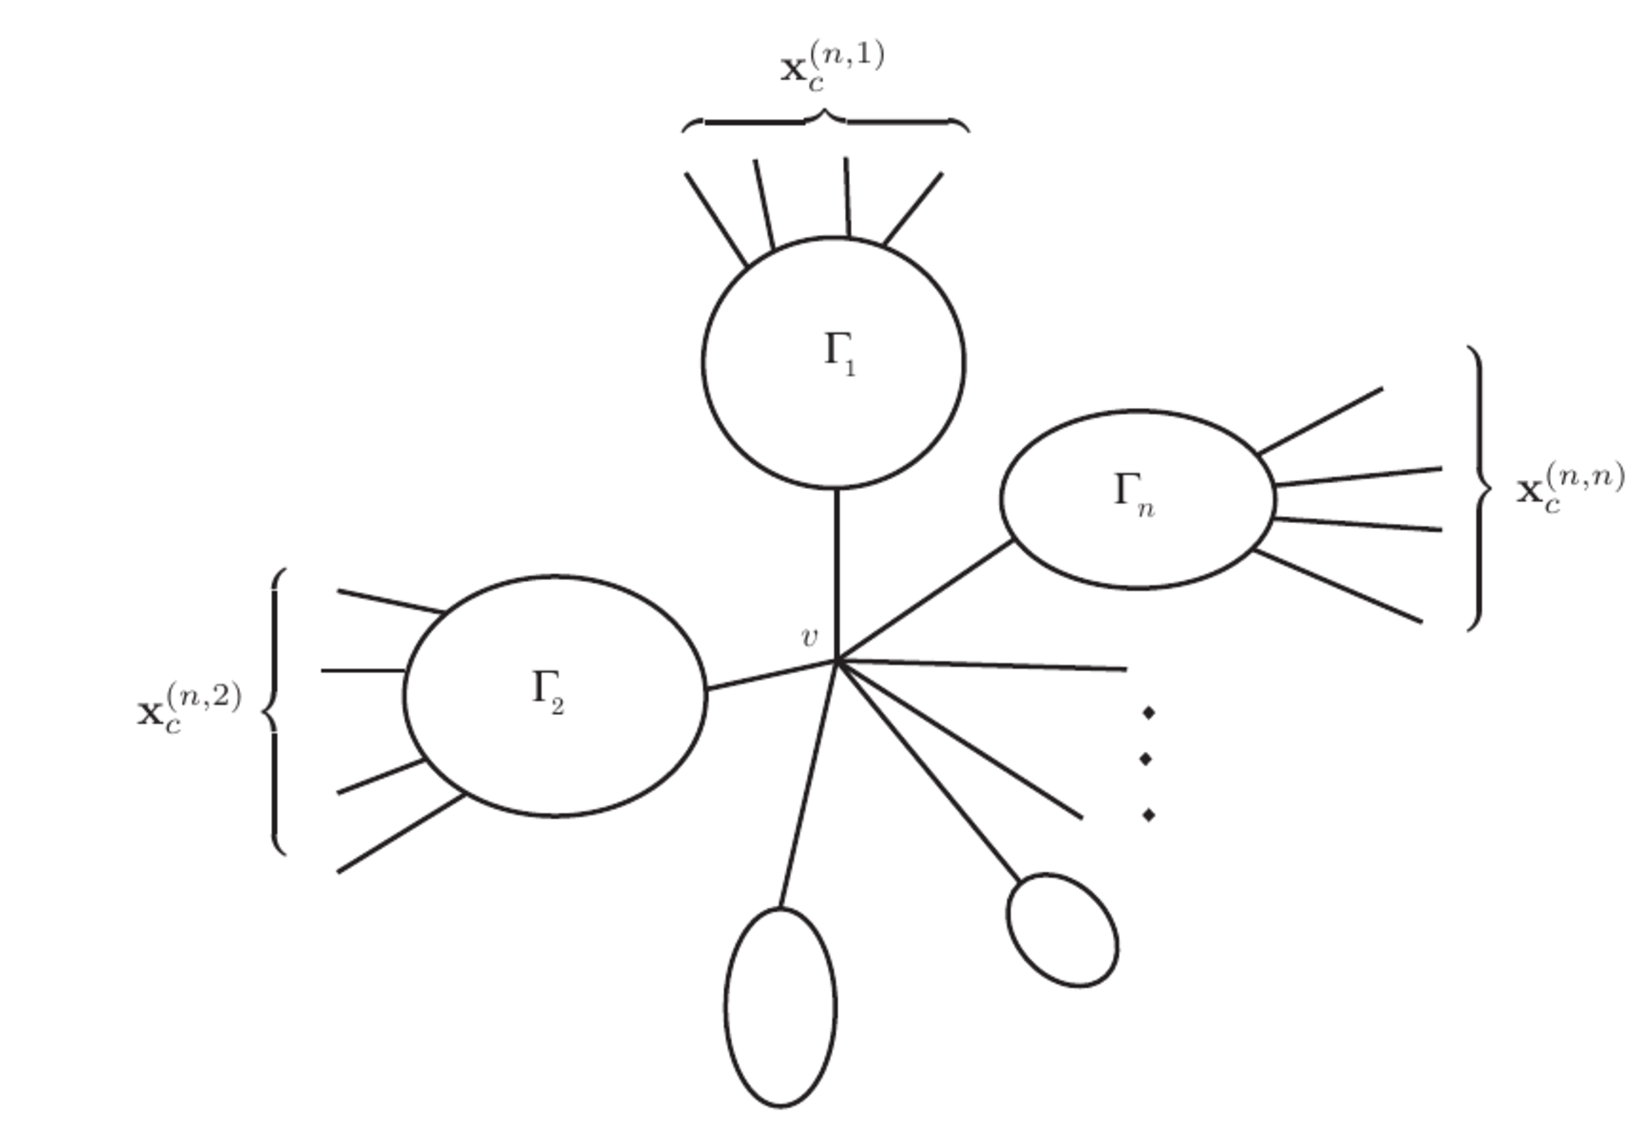
\includegraphics[width=.72\textwidth]{chapters/ch07-transversality/figures/phys-656-figure-7-4-19-final-crop.png}
\par\smallskip
{\renewcommand{\thefigure}{7.4.19}\refstepcounter{figure}
\normalfont\bfseries 图~\thefigure\label{fig:7-4-19}}
\end{minipage}\par\medskip

现在置
\begin{equation}
\begin{aligned}
\mathfrak h_{\ell,n}(\mathbf Y)(V)
=
\sum_{k_1,\ldots,k_n}
\sum_{\mathfrak Y\in\operatorname{Shuff}(\mathbf Y;n)}
\mathfrak h_{\ell;k_1,\ldots,k_n}(\mathfrak Y,V),
\end{aligned}
\tag{7.4.189.1}\label{eq:7-4-189-1}
\end{equation}
以及
\begin{equation}
\mathfrak h^\circ_{\ell,n}(\mathbf Y)(V)
=\mathfrak h_{\ell,n}
\bigl(\operatorname{Op}(\mathbf Y)\bigr)(V).
\tag{7.4.189.2}\label{eq:7-4-189-2}
\end{equation}
仿照定理~\ref{thm:7-4-41} 的证明，
可以证明 $\mathfrak h^\circ$ 是滤过 $L_\infty$ 左模同态，
并且是同伦等价。
定理~\ref{thm:7-4-186} 得证。
\end{proof}
